\documentclass{amsart}

% For revision control
\usepackage{rcs-multi}
\rcsid{$Id$}
\rcsid{$Header$}
\rcskwsave{$Author$}
\rcskwsave{$Date$} 
\rcskwsave{$Revision$}
%%\rcsRegisterAuthor{devangel}{Dennis Jos{\'e} Evangelista}
\rcsRegisterAuthor{devangel}{Dennis J. Evangelista}

\usepackage{graphicx}
\usepackage[usenames,dvipsnames]{color}
%\usepackage{makeidx} % incompatible with ams art
\usepackage{siunitx}
\DeclareMathOperator*{\argmin}{\arg\!\min}
\usepackage{multirow}
\usepackage{colortbl}

% PDF metadata
\usepackage{hyperref}
\hypersetup{pdftitle={Modeling multi-axis zero angular momentum turns the easy way}}
\hypersetup{pdfauthor={Rachel Becker, Dennis Evangelista, and Eliza McDonald}}
\hypersetup{pdfsubject={biology}}
\hypersetup{pdfkeywords={biomechanics, estimation, maneuverability, modeling, angular momentum, turns}}
\hypersetup{colorlinks=true,citecolor=Violet,linkcolor=Blue,urlcolor=Red}


\title{Modeling multi-axis zero angular momentum turns the easy way}
\author{Rachel Becker, Dennis Evangelista, and Eliza McDonald}
\address{Department of Integrative Biology, UC Berkeley}
\email{devangel@berkeley.edu}
\thanks{Tom Daniel first suggested to me the idea of predicting what an animal would do if there were no air, in the solely inertial case.}
\date{\today}

\begin{document}
\begin{abstract}
These notes give our thoughts on how to numerically test a recorded movement for use of zero- and constant angular momentum turning mechanics. 
\end{abstract}
\maketitle
\tableofcontents

\section{Introduction}
We wish to examine the earliest instants of roll, pitch, and yaw maneuvers made by baby birds (Chukar Partridge (\emph{Alectoris chukar}) and Mallard Duck (\emph{Anas platyrhynchos}), from \SI{1}{dph} to fledging).  At this early age, the wings are not yet fully developed.  In addition, during the initial instants of a fall, the body has not yet attained sufficient airspeed to develop large aerodynamic forces and torques, which scale $\sim \rho U^2 A$ and $\rho U^2 A \lambda$, respectively.  Consequently we might expect these early maneuvers to involve significant contribution from other mechanisms, such as inertial mechanisms \cite{Edwards:1986, Jusufi:2008, Jusufi:2010}.  Inertial mechanisms are ones in which body angular position is changed by modulating body inertia, either to modulate some initial angular momentum obtained when leaving the ground, or to effect a zero- or constant angular momentum turn \cite{Edwards:1986}.  In order to answer questions of biological interest, we need general ways (numerical methods) to test if a given maneuver uses inertial mechanisms or detect when non-inertial mechanisms must be at work. 






\subsection{Conservation of angular momentum $H$}
First, some definitions are in order.  For a collection of moving particles, we can define angular momentum about an arbitrary point $B$ as follows (after \cite{Baruh:1999}):
\begin{equation}
\vec{H}_B = \sum_i \vec{r}_{Bi} \times m_i \vec{v}_i
\end{equation}
We also introduce the centroid, or center of mass $G$: 
\begin{equation}
\vec{r}_G = \frac{\sum_i m_i \vec{r}_i}{\sum_i m_i}
\label{eq:COM}
\end{equation}
which, for our collection of moving particles, may also be moving.  The angular momentum about the center of mass reduces to a convenient form:
\begin{equation}
\frac{d}{dt} \vec{H}_G = \vec{M}_G
\end{equation}
where $M_G$ are the externally applied moments about the center of mass. In the case of an organism in free fall, where it has not yet attained sufficient speed for aerodynamic torques to be significant, and is not ejecting any mass or in contact with things that it can push off on (refer to \cite{Baruh:1999} for the derivation of this result) 
\begin{equation}
\frac{d}{dt} \vec{H}_G = 0
\end{equation}
or alternatively,
\begin{equation}
\vec{H}_G = \sum_i \vec{r}_{Gi} \times m_i \vec{v}_i = \mbox{constant}
\label{eq:zam}
\end{equation}
In other words, angular momentum is conserved.  

Equation~\ref{eq:zam} will be the main tool we use in our simulations and analyses in two ways.  First, we will take observations of body position and calculate $H_G$, to test if angular momentum is constant and detect if a maneuver requires use of external (aerodynamic) torques. This first task is easy.  Second, given a sequence of body positions in coordinates fixed to the body, we should be able to project what whole-body rotations should result in the absence of air, i.e.\ if the animal were magically flying in a vacuum.  The second task is only a little harder. 






\subsection{Calculating $H$ from observed positions, the easy way}
\label{sec:forward}
By filming an organism with multiple calibrated cameras, it is often possible to obtain estimates of three-dimensional position for joints, markers, limbs, etc.  We denote these measured positions as a set of position vectors in the rest frame $\vec{r}_{0i}[n]$, where $[n]$ represents each discrete time frame of the video.  

With each point we will also associate a point mass $m_i$ representing the mass of each chunk of the organism. This is a simplification; organisms are not point masses in general, but small chunks of an animal can be approximated as such to simplify calculation\footnote{We really really really wish to avoid dealing with long kinematic chains where each link has large inertia; any more than two links is very hard to write and likely to induce madness.}. We can guess $m_i$ from the shape of the animal, or by using a good balance and a meat cleaver. Unless chunks of the organism are removed or redistributed during the sequence (not usually the case for terrestrial animals), $m$ does not depend on time $[n]$. Thus, our analysis model of the organism is a system of point masses with prescribed motions.  

To numerically calculate the angular momentum $H$ of the system, we proceed by finding the location of the center of mass $\vec{r}_G$ using Equation~\ref{eq:COM} above. We subtract to find the time-varying body positions relative to the time-varying center of mass:
\begin{equation}
\vec{r}_{Gi}[n] = \vec{r}_{0i}[n]-\vec{r}_{G}[n]
\label{eq:rg}
\end{equation}
The velocity of each point mass, $\vec{v}_{Gi}[n]$, can be estimated using a simple backwards difference:
\begin{equation}
\vec{v}_{Gi}[n] \approx \frac{\vec{r}_{Gi}[n] - \vec{r}_{Gi}[n-1]}{\Delta t}
\end{equation}
where $\Delta t = 1/\mbox{fps}$ is the period between frames. Taking derivatives of positional data injects noise, but this is the only derivative we need to take, and hopefully it's not as bad as differentiating twice to get accelerations\footnote{If this does turn out to be bad, there are other tricks we can try like spline smoothing or using more explicit models of the body. This is one of those we'll cross our fingers and hope it's OK situations.}. 

We now have all the pieces needed to compute $H_G$ at each time step $[n]$, repeated here: 
\begin{equation}
\vec{H}_{Gi}[n] = \vec{r}_{Gi}[n] \times m_i \vec{v}_{Gi}[n]
\end{equation}
\begin{equation}
\vec{H}_{G}[n] = \sum_i \vec{H}_{Gi}[n]
\end{equation}

For a zero- or constant angular momentum (inertial) maneuver, $H_G[n]$ should be constant, while for a maneuver where external aerodynamic torques are important, $H_G[n]$ will vary with time. Plotting should suffice to tell, or this could be formally tested using maximum likelihood estimation plus an Akaike Information Criterion \cite{notes:tdd}. 

The principal advantage of this numerical formulation is that it is easier to apply to more generalized shapes (e.g.\ a baby bird with two kicking legs, two flapping wings, wagging tail and a head on a long neck; insect with six legs) compared to analytical models of chains of inertias that must be specifically derived for each body plan \cite{Jusufi:2008, Jusufi:2010, Evangelista:unpub2} and which are usually only tractable for small numbers of links.  Kinematics studies naturally produce positions of points, which can easily be used to generate clouds of point masses that track the movements of the study organism and allow computation of its angular momentum. 






\subsection{Predicting body rotation to maintain $H$ constant}
\label{sec:reverse}
We may wish to go the ``opposite'' way in our numerical analysis, in other words, find the expected motions if the maneuver was only inertial.  In this case what we do is a little different.  We begin as before, with a set of position vectors $\vec{r}_{0i}[n]$ for each joint/marker/limb/point as it moves through time $[n]$. We also assume or measure the mass associated with each chunk $m_i$, and we compute the time-varying position of the center of mass $\vec{r}_G$ (Equation~\ref{eq:COM}). From this we use Equation~\ref{eq:rg} to obtain $\vec{r}_{Gi}[n]$, the time-varying body positions relative to the center of mass. So far this is the same as in Section~\ref{sec:forward}. 

In Section~\ref{sec:forward}, we computed $\vec{r}_{Gi}[n]$ in a reference frame that is translating with the center of mass but is not rotating.  Consider instead a reference frame$'$ that translates with the center of mass and also rotates with some logical body-fixed axes, such as in an anatomically bilaterally symmetric animal (antero-posterior, lateral, and dorso-ventral axes)\footnote{It need not be strictly bilaterally symmetric in the posture taken during the maneuver.}.  We denote the body position in the new frame$'$ as:
\begin{equation}
\vec{r}'_{Gi}[n] = \mathbf{R}[n] \cdot \vec{r}_{Gi}[n]
\label{eq:rotation}
%\label{eq:start-reverse}
\end{equation}
where $\mathbf{R}[n]$ is an appropriately chosen, invertible rotation matrix. With the body positions in the new coordinate system, we continue as before to obtain the velocities and ``apparent'' angular momentum:
\begin{equation}
\vec{v}'_{Gi}[n] \approx \frac{\vec{r}'_{Gi}[n] - \vec{r}'_{Gi}[n-1]}{\Delta t}
\end{equation}
\begin{equation}
\vec{H}'_{Gi}[n] = \vec{r}'_{Gi}[n] \times m_i \vec{v}'_{Gi}[n]
\label{eq:fakeH}
\end{equation}
\begin{equation}
\vec{H}'_{G}[n] = \sum_i \vec{H}'_{Gi}[n]
\label{eq:apparent}
\end{equation}
For an inertial maneuver, $H'_G[n]$ will usually \emph{not} be constant because we removed the whole-body rotation when we transformed to a coordinate frame that rotates with the body. Using this discrepancy, we can find the whole-body rotation that would have made the ``real'' angular momentum $H_G$ constant. 

Recall that the ``real'' angular momentum for the case of no external torques $H_{Gi}[n]$ is given by
\begin{equation}
\vec{H}_{G}[n] = \sum_i \vec{r}_{Gi}[n] \times m_i \vec{v}_{Gi}[n] = \mbox{constant} = \vec{H}_G[0]
\end{equation}
Since $\mathbf{R}$ is invertible\footnote{In the case of a body with zero initial angular momentum ($\vec{H}_G[0] = 0$) we can avoid calculating $\mathbf{R}$ entirely! Win!}, we can expand using Equation~\ref{eq:rotation}, keeping in mind that the velocities of each mass also include a component from the whole-body rotation:
\begin{equation}
\vec{H}_{G}[n] = \sum_i \mathbf{R}^{-1}[n] \cdot \vec{r}'_{Gi}[n] \times m_i (\vec{v}'_{Gi}[n] + \vec\omega_G[n] \times \vec{r}'_{Gi}[n] ) = \vec{H}_G[0]
\end{equation}
We then rearrange terms and simplify: 
\begin{equation}
\sum_i \vec{r}'_{Gi}[n] \times m_i (\vec{v}'_{Gi}[n] + \vec\omega_G[n] \times \vec{r}'_{Gi}[n]) = 
\mathbf{R}[n] \cdot \vec{H}_G[0] 
\end{equation}
\begin{equation}
\sum_i \vec{r}'_{Gi}[n] \times m_i \vec{v}'_{G,i}[n] + 
\sum_i \vec{r}'_{Gi}[n] \times m_i \vec\omega_G[n] \times \vec{r}'_{Gi}[n] = 
\mathbf{R}[n] \cdot \vec{H}_G[0] 
\end{equation}
\begin{equation}
\vec{H}'_G[n] +
\mathbf{J}'_G[n] \vec\omega_G[n] = \mathbf{R}[n] \cdot \vec{H}_G[0] 
\end{equation}
\begin{equation}
\vec\omega_G[n] = 
\mathbf{J}_G^{\prime -1}[n] \cdot (\mathbf{R}[n] \cdot \vec{H}_G[0]
-\vec{H}'_G[n]) 
\label{eq:end-reverse}
\end{equation}
where $\mathbf{J}'_G[n]$ are the instantaneous moments of inertia of the body about the body-fixed ($'$) axes and $\vec\omega_G[n]$ is the whole-body rotational speed. It is worthwhile to write out $\mathbf{J}'_G[n]$ and equation~\ref{eq:end-reverse} for the case of zero initial angular momentum ($\vec{H}_G[0]=0$). 
\begin{equation}
\vec\omega_G[n] = 
- \mathbf{J}_G^{\prime -1}[n] \cdot 
\vec{H}'_G[n] 
\label{eq:end-reverse1}
\end{equation}
\begin{equation}
\mathbf{J}'_G[n] = 
\sum_i \begin{bmatrix}
m_i (r_{iy}^2+r_{iz}^2) & -m_i r_{ix} r_{iy} & -m_i r_{ix} r_{iz} \\
-m_i r_{ix} r_{iy} & m_i (r_{ix}^2+r_{iz}^2) & -m_i r_{iy} r_{iz} \\
-m_i r_{ix} r_{iz} & -m_i r_{iy} r_{iz} & m_i (r_{ix}^2+r_{iy}^2) 
\end{bmatrix}
\label{eq:Jn}
\end{equation}
where all $\vec{r}_i$ are evaluated at time $[n]$.  

Using equations~\ref{eq:end-reverse1}, \ref{eq:Jn}, and \ref{eq:apparent}, we can numerically integrate $\vec\omega_G[n]$ to find $\vec\theta_G[n]$, the angular position of the body, and then construct a new rotation matrix $\mathbf{A}[n]$ to rotate the entire body to the new predicted orientation.  We also translate the center of mass according to which external conservative forces (e.g.\ gravity) are acting.

Equations~\ref{eq:end-reverse1}, \ref{eq:Jn}, and \ref{eq:apparent} allow us to predict the overall motion of a body given prescribed appendage movements (flapping, kicking, tail wagging) with respect to body-fixed coordinates.  To be sure the numerical methods work correctly, we can check these methods and those from Section~\ref{sec:forward} using simple toy model simulations (Section~\ref{sec:toy}) and actual measured data (Section~\ref{sec:real}). 

\section{Simulation of a two-dimensional toy model}
\label{sec:toy}

\begin{figure}
A 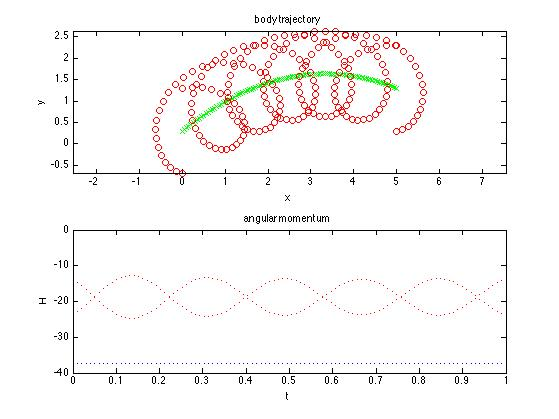
\includegraphics[width=0.4\textwidth]{figures/untitled.jpg}
B 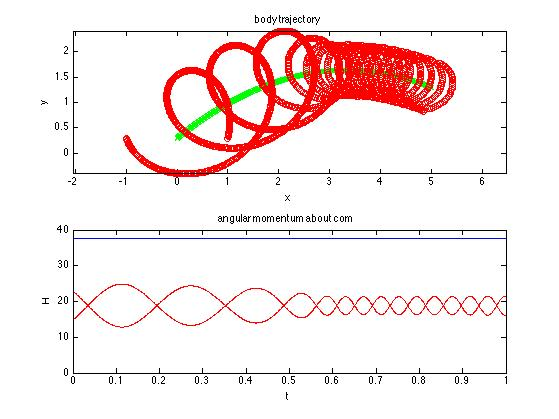
\includegraphics[width=0.4\textwidth]{figures/zam-fling.jpg} \\
C 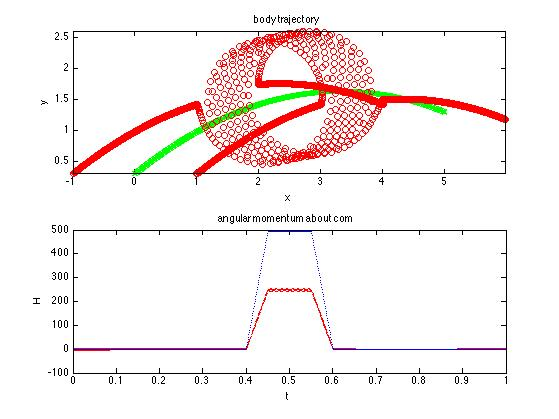
\includegraphics[width=0.4\textwidth]{figures/nonzam-fling.jpg}
D 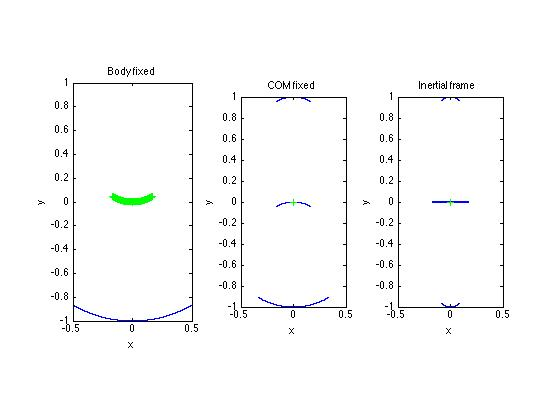
\includegraphics[width=0.4\textwidth]{figures/zam-joint-pos.jpg}

\caption{A. Tumbling amphipod with constant length body showing constant total angular momentum. B. Tumbling amphipod with body shortening at time $t=0.4$, showing rotational speed up to maintain constant total angular momentum. C. Tumbling amphipod with rocket motors firing at time $t=0.4$ and retro-rockets at $t=0.6$, showing non-constant total angular momentum. D. Two-link ``gecko'' with lateral tail wagging \ang{\pm 30} at \SI{3}{\hertz} in body-fixed coordinates (left) and with projected motion assuming zero total angular momentum (right).}
\label{fig:toysim}
\end{figure}

\subsection{Constant angular momentum case}
\subsection{Non-constant angular momentum case}
\subsection{Inertial yawing of a two-link ``gecko''}

%This is an example of a table:
%\begin{table}
%\caption{Hello world in table form.}
%\label{tab:hello}
%\begin{tabular}{lr}
%Able & Baker \\
%Charle & Dog \\
%\end{tabular}
%\end{table}

\section{Results from actual measured kinematics}
\label{sec:real}

\subsection{Real amphipod pitch in yaw, 2-D}
\subsection{Gecko roll from Full lab}
\subsection{Hummingbird yaw maneuver - should be nonZAM} 
\subsection{Diver or skydiver pitching and rolling?}


\section{Conclusions}

% AMS style references
\bibliographystyle{amsplain}
\bibliography{references/modeling-turns}
\end{document}
